\documentclass[main_ppt.tex]{subfiles}
%\documentclass{article}

    % UNITS
%\usepackage{siunitx}
%\sisetup{per=slash, load=abbr}

    % GRAPHICS
%\usepackage{tikz}
%\usepackage{pgfplots}
%\pgfplotsset{width=8cm,height=4cm,compat=newest}

\begin{document}


\begin{columns}

\column{0.8\textwidth}

\pgfplotsset{width=9cm,height=3cm,compat=1.16}
\begin{tikzpicture}
\begin{axis}[
%title= Plot of W displacement VS Time,
axis x line = bottom,
axis y line = left,
xlabel={$Time (s)$},
ylabel={w at y=0},
xmin=0, xmax=5,
%minor y tick num=1,
%legend pos=outer north east,
%cycle list name = color list,
%transpose legend,
%legend columns=3,
%legend style={at={(0.5,-0.1)},anchor=north},
]

%\addplot table{PN2.txt};
%\addplot [blue] table{1E11/Dynamic_Rad_Pn2.txt};
\addplot [blue] table{ParaStudy_onlydata/RandomLoad/Load2.txt};
%\addlegendentry{$SR$ = 1, ST = 2s}


\end{axis}
\end{tikzpicture}



\pgfplotsset{width=9cm,height=3cm,compat=1.16}
\begin{tikzpicture}
\begin{axis}[
%title= Plot of W displacement VS Time,
axis x line = bottom,
axis y line = left,
xlabel={$Time (s)$},
ylabel={w at y=0.5},
xmin=0, xmax=5,
%minor y tick num=1,
%legend pos=outer north east,
%cycle list name = color list,
%transpose legend,
%legend columns=3,
%legend style={at={(0.5,-0.1)},anchor=north},
]

%\addplot table{PN2.txt};
%\addplot [blue] table{1E11/Dynamic_Rad_Pn2.txt};
\addplot [blue] table{ParaStudy_onlydata/RandomLoad/Load1.txt};
%\addlegendentry{$SR$ = 1, ST = 2s}


\end{axis}
\end{tikzpicture}



\pgfplotsset{width=9cm,height=3cm,compat=1.16}
\begin{tikzpicture}
\begin{axis}[
%title= Plot of W displacement VS Time,
axis x line = bottom,
axis y line = left,
xlabel={$Time (s)$},
ylabel={w at y=1},
xmin=0, xmax=5,
%minor y tick num=1,
%legend pos=outer north east,
%cycle list name = color list,
%transpose legend,
%legend columns=3,
%legend style={at={(0.5,-0.1)},anchor=north},
]

%\addplot table{PN2.txt};
%\addplot [blue] table{1E11/Dynamic_Rad_Pn2.txt};
\addplot [blue] table{ParaStudy_onlydata/RandomLoad/Load3.txt};
%\addlegendentry{$SR$ = 1, ST = 2s}


\end{axis}
\end{tikzpicture}

\column{0.2\textwidth}
\href{run:ParaStudy_onlydata/RandomLoad/Dynamic_Rad1.mpg}{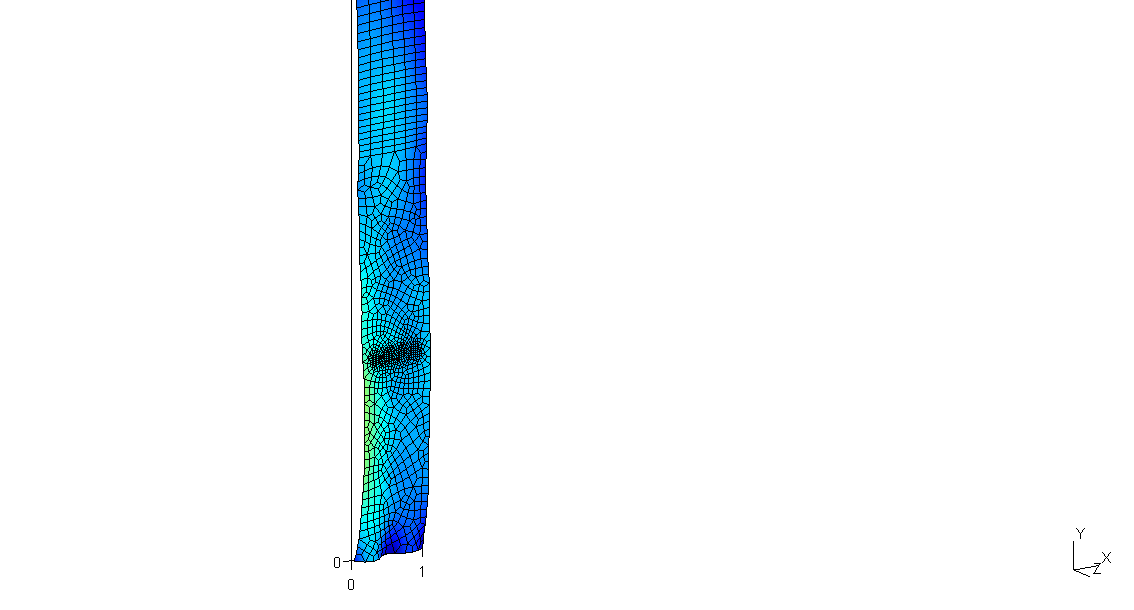
\includegraphics[width=1.0\textwidth,trim={11cm 0cm 22cm 0cm},clip]{ParaStudy_onlydata/RandomLoad/Dynamic_Rad1.png}}
\end{columns}


\end{document}